\documentclass{standalone}
\usepackage{tikz}
\usepackage{amsmath,dsfont}
\usetikzlibrary{automata,positioning,arrows,shapes.geometric, calc,patterns}

\begin{document}
	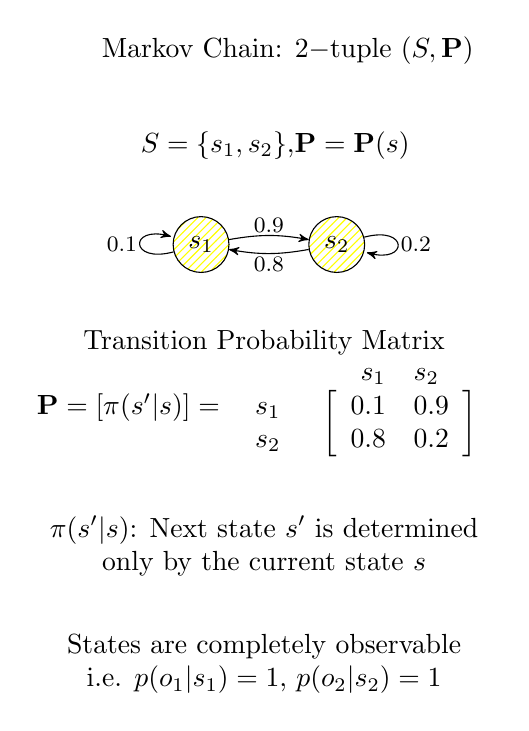
\begin{tikzpicture}[
		shaded/.style={draw,circle,pattern=north east lines, pattern color=yellow},
		> = stealth',
		auto,
		prob/.style = {inner sep=1pt,font=\footnotesize}
		]
		% Markov Chain
		\node[shaded] at (0,0) (s1) {$s_1$};
		\node[shaded, right= of s1] (s2) {$s_2$};
		% Draw the causality arrows
		\path[->] 	(s1) edge [loop left] node[prob] {$0.1$}(s1)
		(s2) edge [loop right] node[prob] {$0.2$}(s2)
		(s1) edge [bend left=10] node[prob]{$0.9$} (s2)
		(s2) edge [bend left = 10] node[prob] {$0.8$}(s1);
		
		% denote
		\node[above = of s1,align=center,xshift= 10mm,yshift = -4mm] (S){ $\mathds{S} = \{s_1,s_2\}$,$\mathbf{P} = \mathbf{P}(s)$ };
		
		\node[above = of S,align=center,xshift= 1mm,yshift = -4mm]  {Markov Chain: $2-$tuple $(\mathds{S},\mathbf{P})$};
		%\node[above = of s1,align=center,xshift= 1mm,yshift = -4mm]  {Markov Chain};
		\node[below = of s1,align=center,xshift= 8mm,yshift = 4mm] (TP)  { Transition Probability Matrix \\$
			\mathbf{P} = [\pi(s'|s)] =
			\begin{array}{cc}
				& \begin{array}{cc} s_1 & s_2 \end{array} \\
				\begin{array}{c}
					s_1 \\
					s_2 \\
				\end{array}
				& \left[ \begin{array}{cc}
					0.1 & 0.9 \\
					0.8 & 0.2  \\
				\end{array} \right]
			\end{array}
			$};
		\node[below= of TP,align=center,xshift= 0mm,yshift = 5mm] (next) {$\pi(s'|s)$: Next state $s'$ is determined \\ only by the current state $s$};
		\node[below= of next,align=center,xshift= 0mm,yshift = 5mm] (next) {States are completely observable\\i.e. $p(o_1|s_1) = 1$, $p(o_2|s_2) = 1$};	
	\end{tikzpicture}
	
	% Hidden Markov Model
	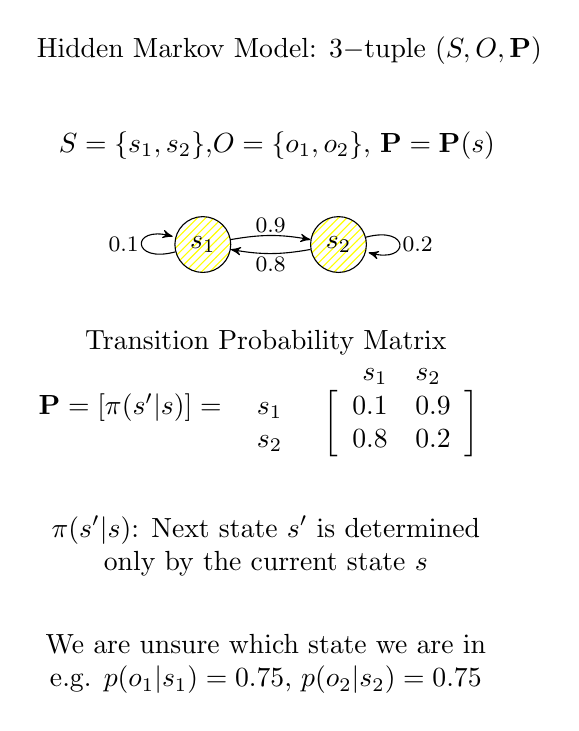
\begin{tikzpicture}[
		shaded/.style={draw,circle,pattern=north east lines, pattern color=yellow},
		> = stealth',
		auto,
		prob/.style = {inner sep=1pt,font=\footnotesize}
		]
		\node[shaded] at (0,0) (s1) {$s_1$};
		\node[shaded, right= of s1] (s2) {$s_2$};
		% Draw the causality arrows
		\path[->] 	(s1) edge [loop left] node[prob] {$0.1$}(s1)
		(s2) edge [loop right] node[prob] {$0.2$}(s2)
		(s1) edge [bend left=10] node[prob]{$0.9$} (s2)
		(s2) edge [bend left = 10] node[prob] {$0.8$}(s1);
		
		% denote
		%\node[above = of s1,align=center,xshift= 1mm,yshift = -4mm]  {Hidden Markov Model};
		\node[above = of s1,align=center,xshift= 10mm,yshift = -4mm] (S){ $\mathds{S} = \{s_1,s_2\}$,$\mathds{O} = \{o_1,o_2\}$, $\mathbf{P} = \mathbf{P}(s)$ };
		
		\node[above = of S,align=center,xshift= 1mm,yshift = -4mm]  {Hidden Markov Model: $3-$tuple $(\mathds{S},\mathds{O},\mathbf{P})$};
	
		\node[below = of s1,align=center,xshift= 8mm,yshift = 4mm] (TP)  {Transition Probability Matrix \\$
			\mathbf{P} =  [\pi(s'|s)] =
			\begin{array}{cc}
				& \begin{array}{cc} s_1 & s_2 \end{array} \\
				\begin{array}{c}
					s_1 \\
					s_2 \\
				\end{array}
				& \left[ \begin{array}{cc}
					0.1 & 0.9 \\
					0.8 & 0.2  \\
				\end{array} \right]
			\end{array}
			$};
		\node[below= of TP,align=center,xshift= 0mm,yshift = 5mm] (next) {$\pi(s'|s)$: Next state $s'$ is determined \\ only by the current state $s$};
		\node[below= of next,align=center,xshift= 0mm,yshift = 5mm] (next) {We are unsure which state we are in \\e.g. $p(o_1|s_1) = 0.75$, $p(o_2|s_2) = 0.75$};	
	\end{tikzpicture}
	
	% Markov Decision Process
	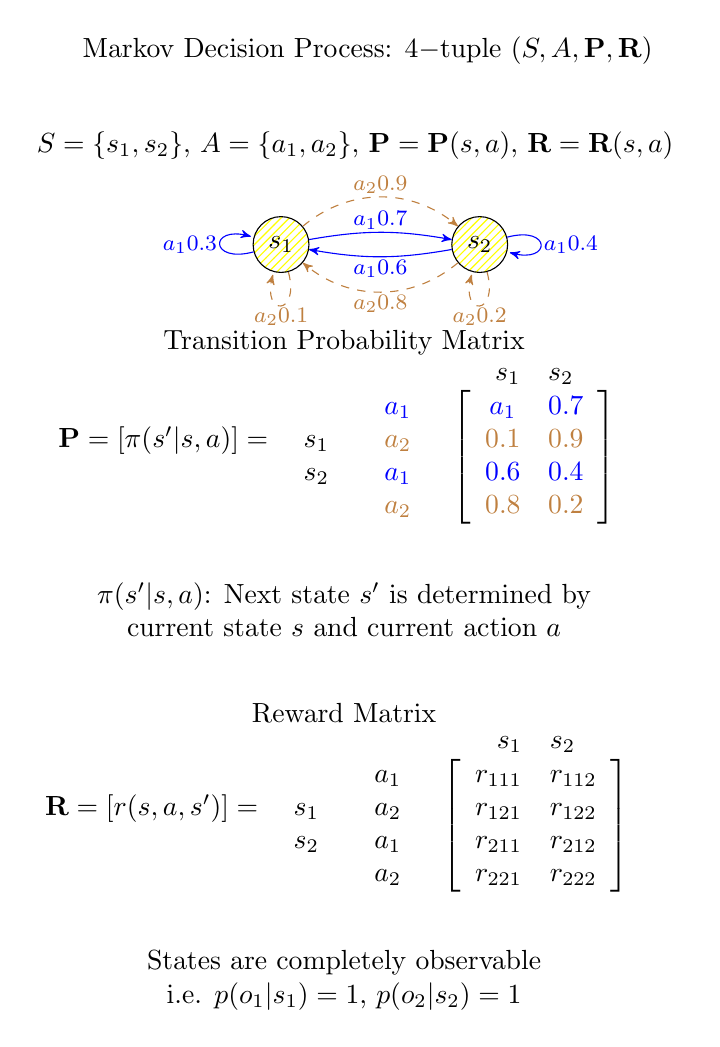
\begin{tikzpicture}[
		shaded/.style={draw,circle,pattern=north east lines, pattern color=yellow},
		> = stealth',
		auto,
		prob/.style = {inner sep=1pt,font=\footnotesize}
		]
		\node[shaded] at (0,0) (s1) {$s_1$};
		\node[shaded, right= of s1,xshift= 8mm] (s2) {$s_2$};
		% Draw the causality arrows
		\path[->] 	
		(s1) edge [loop left,blue] node[prob] {$a_1 0.3$}(s1)
		(s1) edge [loop below,brown,dashed] node[prob] {$a_2 0.1$}(s1)
		(s2) edge [loop right,blue] node[prob] {$a_1 0.4$}(s2)
		(s2) edge [loop below,brown,dashed] node[prob] {$a_2 0.2$}(s2)
		(s1) edge [bend left=10,blue] node[prob]{$a_1 0.7$} (s2)
		(s1) edge [bend left = 40,brown,dashed] node[prob]{$a_2 0.9$} (s2)
		(s2) edge [bend left = 10,blue] node[prob] {$a_1 0.6$}(s1)
		(s2) edge [bend left = 40,brown,dashed] node[prob] {$a_2 0.8$}(s1);
		
		% denote
		\node[above = of s1,align=center,xshift= 10mm,yshift = -4mm] (S){ $\mathds{S} = \{s_1,s_2\}$, $\mathds{A} = \{a_1,a_2\}$,
		$\mathbf{P} = \mathbf{P}(s,a)$, $\mathbf{R} = \mathbf{R}(s,a)$ };
		
		\node[above = of S,align=center,xshift= 1mm,yshift = -4mm]  {Markov Decision Process: $4-$tuple $(\mathds{S},\mathds{A},\mathbf{P},\mathbf{R})$};
		
		\node[below = of s1,align=center,xshift= 8mm,yshift = 4mm] (TP)  { Transition Probability Matrix \\$
			\mathbf{P}  = [\pi(s'|s,a)] = 
			\begin{array}{ccc}
				&  &\begin{array}{cc} s_1 & s_2 \end{array} \\
				\begin{array}{c}
					s_1 \\
					s_2 
				\end{array} 
				&
				\begin{array}{c}
					\textcolor{blue}{a_1} \\
					\textcolor{brown}{a_2} \\
					\textcolor{blue}{a_1} \\
					\textcolor{brown}{a_2}
				\end{array} 
				& \left[ \begin{array}{cc}
					\textcolor{blue}{a_1}& \textcolor{blue}{0.7}\\
					\textcolor{brown}{0.1} & \textcolor{brown}{0.9} \\
					\textcolor{blue}{0.6} & \textcolor{blue}{0.4} \\
					\textcolor{brown}{0.8} & \textcolor{brown}{0.2}  
				\end{array} \right]
			\end{array}
			$};
		\node[below= of TP,align=center,xshift= 0mm,yshift = 5mm] (next) { $\pi(s'|s,a)$: Next state $s'$ is determined by \\ current state $s$ and current action $a$};
		\node[below = of next,align=center,xshift= 0mm,yshift = 4mm] (reward)  { Reward Matrix \\$
			\mathbf{R}  = [r(s,a,s')] =
			\begin{array}{ccc}
				&  &\begin{array}{cc} s_1 & s_2 \end{array} \\
				\begin{array}{c}
					s_1 \\
					s_2 
				\end{array} 
				&
				\begin{array}{c}
					a_1 \\
					a_2 \\
					a_1 \\
					a_2
				\end{array} 
				& \left[ \begin{array}{cc}
					r_{111} & r_{112} \\
					r_{121} & r_{122} \\
					r_{211} & r_{212}\\
					r_{221} & r_{222} 
				\end{array} \right]
			\end{array}
			$};
		\node[below= of reward,align=center,xshift= 0mm,yshift = 5mm] (next) {States are completely observable\\i.e. $p(o_1|s_1) = 1$, $p(o_2|s_2) = 1$};	
	\end{tikzpicture}

	% Partially Observable Markov Decision Process
	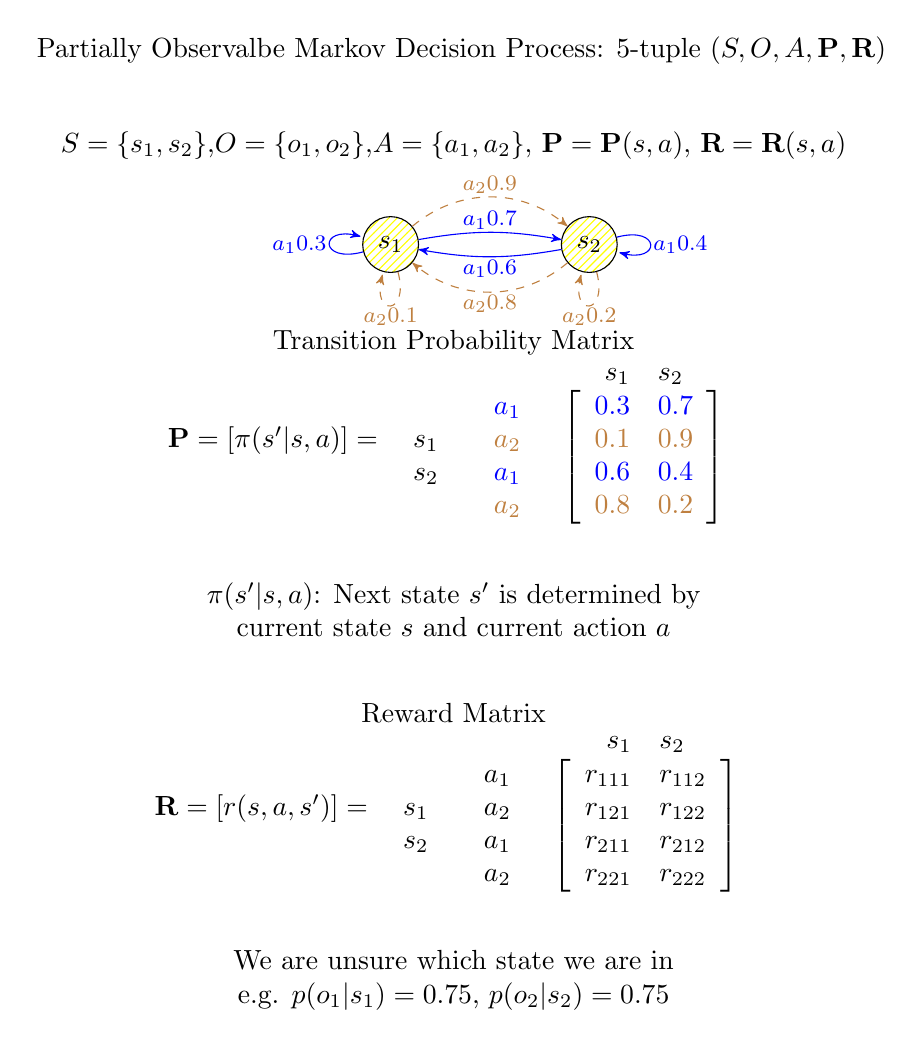
\begin{tikzpicture}[
		shaded/.style={draw,circle,pattern=north east lines, pattern color=yellow},
		> = stealth',
		auto,
		prob/.style = {inner sep=1pt,font=\footnotesize}
		]
		\node[shaded] at (0,0) (s1) {$s_1$};
		\node[shaded, right= of s1,xshift= 8mm] (s2) {$s_2$};
		% Draw the causality arrows
		\path[->] 	
		(s1) edge [loop left,blue] node[prob] {$a_1 0.3$}(s1)
		(s1) edge [loop below,brown,dashed] node[prob] {$a_2 0.1$}(s1)
		(s2) edge [loop right,blue] node[prob] {$a_1 0.4$}(s2)
		(s2) edge [loop below,brown,dashed] node[prob] {$a_2 0.2$}(s2)
		(s1) edge [bend left=10,blue] node[prob]{$a_1 0.7$} (s2)
		(s1) edge [bend left = 40,brown,dashed] node[prob]{$a_2 0.9$} (s2)
		(s2) edge [bend left = 10,blue] node[prob] {$a_1 0.6$}(s1)
		(s2) edge [bend left = 40,brown,dashed] node[prob] {$a_2 0.8$}(s1);
		
		% denote
		\node[above = of s1,align=center,xshift= 8mm,yshift = -4mm](S)  {$\mathds{S} = \{s_1,s_2\}$,$\mathds{O} = \{o_1,o_2\}$,$\mathds{A} = \{a_1,a_2\}$, $\mathbf{P} = \mathbf{P}(s,a)$, $\mathbf{R} = \mathbf{R}(s,a)$};
		\node[above = of S,align=center,xshift= 1mm,yshift = -4mm]  {Partially Observalbe Markov Decision Process: 5-tuple $(\mathds{S},\mathds{O},\mathds{A},\mathbf{P},\mathbf{R})$};
		\node[below = of s1,align=center,xshift= 8mm,yshift = 4mm] (TP)  { Transition Probability Matrix \\$
			\mathbf{P}  = [\pi(s'|s,a)] =
			\begin{array}{ccc}
				&  &\begin{array}{cc} s_1 & s_2 \end{array} \\
				\begin{array}{c}
					s_1 \\
					s_2 
				\end{array} 
				&
				\begin{array}{c}
					\textcolor{blue}{a_1} \\
					\textcolor{brown}{a_2} \\
					\textcolor{blue}{a_1} \\
					\textcolor{brown}{a_2}
				\end{array} 
				& \left[ \begin{array}{cc}
					\textcolor{blue}{0.3} & \textcolor{blue}{0.7} \\
					\textcolor{brown}{0.1} & \textcolor{brown}{0.9} \\
					\textcolor{blue}{0.6} & \textcolor{blue}{0.4} \\
					\textcolor{brown}{0.8} & \textcolor{brown}{0.2}  
				\end{array} \right]
			\end{array}
			$};
		\node[below= of TP,align=center,xshift= 0mm,yshift = 5mm] (next) { $\pi(s'|s,a)$: Next state $s'$ is determined by \\ current state $s$ and current action $a$};
		\node[below = of next,align=center,xshift= 0mm,yshift = 4mm] (reward)  { Reward Matrix \\$
			\mathbf{R}  = [r(s,a,s')] =
			\begin{array}{ccc}
				&  &\begin{array}{cc} s_1 & s_2 \end{array} \\
				\begin{array}{c}
					s_1 \\
					s_2 
				\end{array} 
				&
				\begin{array}{c}
					a_1 \\
					a_2 \\
					a_1 \\
					a_2
				\end{array} 
				& \left[ \begin{array}{cc}
					r_{111} & r_{112} \\
					r_{121} & r_{122} \\
					r_{211} & r_{212}\\
					r_{221} & r_{222} 
				\end{array} \right]
			\end{array}
			$};
		\node[below= of reward,align=center,xshift= 0mm,yshift = 5mm] (next) {We are unsure which state we are in\\e.g. $p(o_1|s_1) = 0.75$, $p(o_2|s_2) = 0.75$};	
	\end{tikzpicture}
	
	
	
	
			% semi-Markov Decision Process
	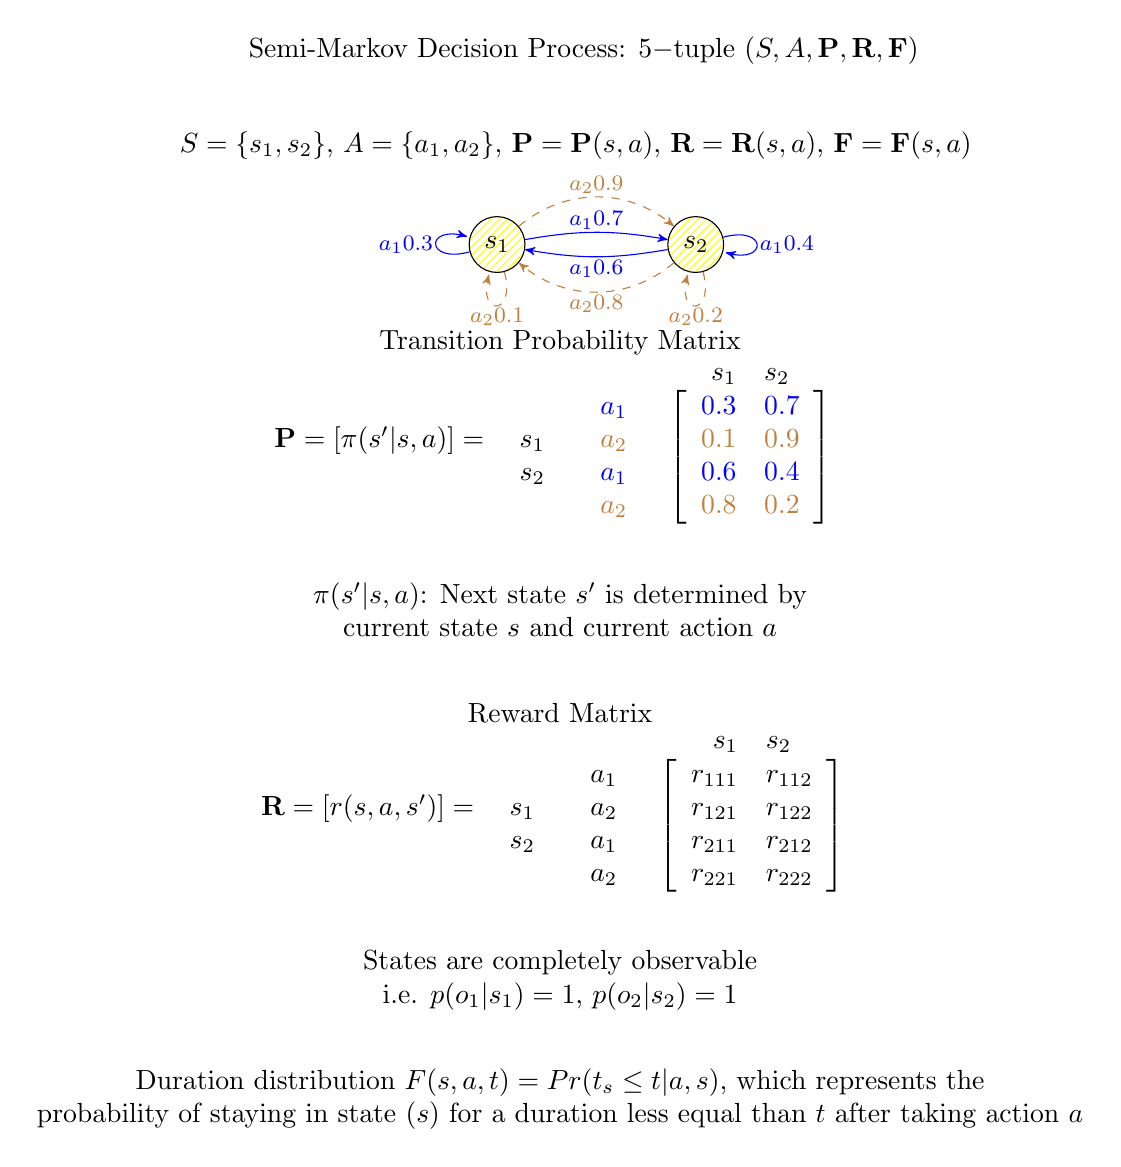
\begin{tikzpicture}[
		shaded/.style={draw,circle,pattern=north east lines, pattern color=yellow},
		> = stealth',
		auto,
		prob/.style = {inner sep=1pt,font=\footnotesize}
		]
		\node[shaded] at (0,0) (s1) {$s_1$};
		\node[shaded, right= of s1,xshift= 8mm] (s2) {$s_2$};
		% Draw the causality arrows
		\path[->] 	
		(s1) edge [loop left,blue] node[prob] {$a_1 0.3$}(s1)
		(s1) edge [loop below,brown,dashed] node[prob] {$a_2 0.1$}(s1)
		(s2) edge [loop right,blue] node[prob] {$a_1 0.4$}(s2)
		(s2) edge [loop below,brown,dashed] node[prob] {$a_2 0.2$}(s2)
		(s1) edge [bend left=10,blue] node[prob]{$a_1 0.7$} (s2)
		(s1) edge [bend left = 40,brown,dashed] node[prob]{$a_2 0.9$} (s2)
		(s2) edge [bend left = 10,blue] node[prob] {$a_1 0.6$}(s1)
		(s2) edge [bend left = 40,brown,dashed] node[prob] {$a_2 0.8$}(s1);
		
		% denote
		\node[above = of s1,align=center,xshift= 10mm,yshift = -4mm] (S){ $\mathds{S} = \{s_1,s_2\}$, $\mathds{A} = \{a_1,a_2\}$,
		$\mathbf{P} = \mathbf{P}(s,a)$,
		$\mathbf{R} = \mathbf{R}(s,a)$,
		$\mathbf{F} = \mathbf{F}(s,a)$};
		
		\node[above = of S,align=center,xshift= 1mm,yshift = -4mm]  {Semi-Markov Decision Process: $5-$tuple $(\mathds{S},\mathds{A},\mathbf{P},\mathbf{R},\mathbf{F})$};
		
		\node[below = of s1,align=center,xshift= 8mm,yshift = 4mm] (TP)  { Transition Probability Matrix \\$
			\mathbf{P}  = [\pi(s'|s,a)] =
			\begin{array}{ccc}
				&  &\begin{array}{cc} s_1 & s_2 \end{array} \\
				\begin{array}{c}
					s_1 \\
					s_2 
				\end{array} 
				&
				\begin{array}{c}
					\textcolor{blue}{a_1} \\
					\textcolor{brown}{a_2} \\
					\textcolor{blue}{a_1} \\
					\textcolor{brown}{a_2}
				\end{array} 
				& \left[ \begin{array}{cc}
					\textcolor{blue}{0.3} & \textcolor{blue}{0.7} \\
					\textcolor{brown}{0.1} & \textcolor{brown}{0.9} \\
					\textcolor{blue}{0.6} & \textcolor{blue}{0.4} \\
					\textcolor{brown}{0.8} & \textcolor{brown}{0.2}  
				\end{array} \right]
			\end{array}
			$};
		\node[below= of TP,align=center,xshift= 0mm,yshift = 5mm] (next) { $\pi(s'|s,a)$: Next state $s'$ is determined by \\ current state $s$ and current action $a$};
		\node[below = of next,align=center,xshift= 0mm,yshift = 4mm] (reward)  { Reward Matrix \\$
			\mathbf{R} =  [r(s,a,s')] =
			\begin{array}{ccc}
				&  &\begin{array}{cc} s_1 & s_2 \end{array} \\
				\begin{array}{c}
					s_1 \\
					s_2 
				\end{array} 
				&
				\begin{array}{c}
					a_1 \\
					a_2 \\
					a_1 \\
					a_2
				\end{array} 
				& \left[ \begin{array}{cc}
					r_{111} & r_{112} \\
					r_{121} & r_{122} \\
					r_{211} & r_{212}\\
					r_{221} & r_{222} 
				\end{array} \right]
			\end{array}
			$};
		\node[below= of reward,align=center,xshift= 0mm,yshift = 5mm] (next) {States are completely observable\\i.e. $p(o_1|s_1) = 1$, $p(o_2|s_2) = 1$};	
		\node[below = of next, align=center,xshift= 0mm,yshift = 5mm] (duration) {Duration distribution $F(s,a,t) = Pr(t_s \leq t|a,s)$, which represents the \\ probability of staying in state $(s)$ for a duration less equal than $t$ after taking action $a$};	
	\end{tikzpicture}
\end{document}
